%!TEX root = ../gesamt.tex

\begin{Satz}{\label{kap_10_satz18}
	Sei $f: [a,b] \rightarrow \mathbb{R}$ beschränkt. Dann ist 
	$f \in \mathcal{R}_{[a,b]}$ genau dann, wenn für jedes $\epsilon > 0$ eine 
	Partition $P_{\epsilon}$ existiert mit:
	\begin{align*}
		S(P_2,f) - s(P_2,f) < \epsilon
	\end{align*}
}\end{Satz}

\begin{proof}
	 Per Definition gilt 
	\begin{align*}
		s(P_{\epsilon},f) \leq \underline{\int_{a}^b} f \dd{x}
		\overset{Satz~\ref{kap09_satz17}}{\le} \overline{\int_a^b} f \dd{x} 
		\leq S(P_{\epsilon},f) 		
	\end{align*}

	Damit erhalten wir:
	\begin{align*}
		\overline{\int_a^b} f \dd{x} - 
		\underline{\int_{a}^b} f \dd{x} \leq S(P_{\epsilon},f) 
		- s(P_{\epsilon},f) < \epsilon
	\end{align*}
	Das heißt, da $\epsilon$ beliebig, dass:
	\begin{align*}
		\underline{\int_{a}^b} \dd{x} = \overline{\int_a^b} f \dd{x}
	\end{align*}
	Ergo: $f \in \mathcal{R}_{[a,b]}$ \\
	Per Definition gibt es für alle $\epsilon > 0$ ein $P_{\epsilon}'$ mit:
	\begin{align}
		\label{gleichung_1_1505}
		\underline{\int_{a}^b} f \dd{x} - s(P_{\epsilon}',f) < \frac{\epsilon}{2} 
	\end{align}
	Analog existiert ein $P_{\epsilon}''$ mit 
	\begin{align}
		\label{gleichung_2_1505}
		S(P_{\epsilon}'',f) - \overline{\int_a^{b}} f \dd{x}) < \frac{\epsilon}{2}
	\end{align}
	Wir setzten $P_{\epsilon}$ gleich der gemeinsamen Vereinigung von 
	$P_{\epsilon}'$ und $P_{\epsilon}''$. Man beachte: Wegen Satz~\ref{kap09_satz16} 
	gelten Gleichung~\ref{gleichung_1_1505} und Gleichung~\ref{gleichung_2_1505},
	wenn wir $P_{\epsilon}'$, beziehungsweise $P_{\epsilon}''$, durch $P_{\epsilon}$
	ersetzen. Da $f \in \mathcal{R}_{[a,b]}$ gilt außerdem:
	\begin{align*}
		\underline{\int_{a}^b} f \dd{x} = \overline{\int_a^{b}} f\dd{x}
	\end{align*}	 
	Addition von Gleichung~\ref{gleichung_1_1505} und Gleichung~
	\ref{gleichung_2_1505} liefert:
	\begin{align*}
	S(P_{\epsilon},f) - s(P_{\epsilon},f) < \epsilon
	\end{align*}
\end{proof}

\begin{Satz}{\label{kap10_satz19}
	Sei $f:[a,b] \rightarrow \mathbb{R}$ beschränkt und $P_{\epsilon} = 
	\{x_0, \hdots, x_n\}$ eine Partition von $[a,b]$ mit $S(P_{\epsilon},f) -
	s(P_{\epsilon},f) < \epsilon$ für ein $\epsilon > 0$.
	\begin{enumerate}
		\item Ist $P$ eine Verfeinerung von $P_{\epsilon}$, so gilt 
		$S(P,f) - s(P,f) < \epsilon$
		\item Sind $s_i, t_i$ beliebige Punkte in $[x_{i-1},x_i]$, so gilt:
		\begin{align*}
			\sum_{i=1}^n \left\vert f(s_i) - f(t_i) \right\vert \cdot 
			\Delta x_i < \epsilon
		\end{align*}
		\item Ist $f \in \mathcal{R}_{[a,b]}$ und $t_i \in [x_{i-1},x_i]$, so 
		gilt 
		\begin{align*}
			\left\vert \sum_{i=1}^n f(t_i) \cdot \Delta x_i - \int_a^b f \dd{x} 
			\right\vert < \epsilon
		\end{align*}
	\end{enumerate}	
}\end{Satz}

\begin{proof}
	\begin{enumerate}
		\item[ ]
		\item Das folgt aus Satz~\ref{kap09_satz16}
		\item
		 \begin{align*}
			\sum_{i = 1}^n \left\vert f(s_i) - f(t_i) \right\vert	\cdot 
			\Delta x_i \leq \sum_{i=1}^n (M_i-m_i)\cdot \Delta x_i
			= S(P_{\epsilon},f) - s(P_{\epsilon},f) < \epsilon
		 \end{align*}
		 \item Da $t_i \in [x_{i-1},x_i]$, gilt $m_i \leq f(t_i) \leq M_i$ \\
		 	Damit folgt die Aussage aus
			 \begin{align*}
			 	s(P_{\epsilon},f ) \leq  
			 	\sum_{i = 1}^n m_i \cdot \Delta x_i \leq \sum_{i=1}^n f(t_i) \cdot \Delta 
			 	x_i \leq \sum_{i=1}^n M_i \cdot \Delta x_i = S(P_{\epsilon},f)
			 \end{align*}
			 und $s(P_{\epsilon},f) \leq \int_a^b f \dd{x} \leq S(P_{\epsilon},f)$
	\end{enumerate}
\end{proof}
	Wir wollen im Folgenden wichtige Vertreter Riemann-integrierbarer 
	Funktionen kennenlernen.

\begin{Satz}{\label{kap10_satz20}
	Ist $f: [a,b] \rightarrow \mathbb{R}$ stetig, so ist 
	$ f \in \mathcal{R}_{[a,b]}$.
}\end{Satz}

\begin{proof}
	Da stetige Funktionen auf abgeschlossenen Intervallen 
	beschränkt sind, ist $f$ offensichtlich beschränkt. Weiterhin ist $f$ als stetige 
	Funktion auf dem abgeschlossenen Intervall $[a,b]$ gleichmäßig stetig. \\
	Sei $\epsilon > 0 $ gegeben. Wegen der gleichmäßigen Stetigkeit von $f$ 
	existiert ein $\delta > 0$, so dass folgende Implikation gilt:
	\begin{align*}
		\vert x - y \vert < \delta \Rightarrow \vert f(x) -f(y) \vert < \epsilon
	\end{align*}
	Wir wählen eine Partition $P_{\epsilon} = \{ x_0, \hdots, x_n \}$, so dass 
	$\Delta x_i < \delta$. Dann gilt:
	\begin{align*}
		M_i - m_i < & \epsilon \text{ und daher} \\
		S(P_{\epsilon},f) - s(P_{\epsilon},f) = & \sum_{i = 1}^n (M_i -m_i)\Delta x_i 
		\leq \epsilon \cdot \sum_{i = 1}^n \Delta x_i = \epsilon \cdot (b-a)
	\end{align*}
	Da $\epsilon > 0$ beliebig, folgt die Aussage mit Satz~\ref{kap_10_satz18}.
\end{proof}

\begin{Satz}{
		Ist $f: [a,b] \rightarrow \mathbb{R}$ monoton, so ist 
		$f \in \mathcal{R}_{[a,b]}$ 
}\end{Satz}

\begin{proof}
	 Da $f$ monoton ist, gilt für alle $x \in [a,b]: f(a) \leq f(x) 
	\leq f(b)$. \\
	Das heißt $f$ ist beschränkt. Zu $n \in \mathbb{N}$ wählen wir eine 
	Partition \linebreak $P_n = \{x_0, \hdots, x_k\}$ mit $\Delta x_i < \frac{1}{n}$.
	\begin{figure}
	\begin{center}
	\tikzsetnextfilename{monotone_fkt_riemann_intbar}
		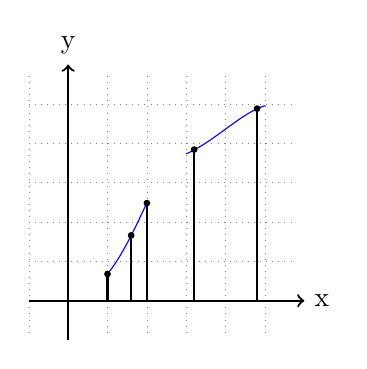
\begin{tikzpicture}
			\draw[dotted, very thin, gray, step = 0.5] (0,-0.9) grid (3.4,2.4);
			
			\draw[->, thick, black](0,-0.5) -- (3.5,-0.5) node[right]{x};
			\draw[->, thick, black](0.5, -1) -- (0.5, 2.5) node[above]{y};
			\draw[blue, domain = 1 :1.5, samples = 1000]  
				plot(\x, {\x * \x * sin(\x r) - \x });
			
			\draw[blue, domain = 2 :3, samples = 1000]  
				plot(\x, {\x * \x * sin(0.5*\x r) - \x*\x + 2});	
			
			\draw[fill=black](1,-0.16)circle(1pt);
			\draw[fill = black](1.3,0.33) circle(1pt);
			\draw[fill = black] (1.5, 0.74) circle(1pt);
			\draw[thick, black](1,-0.5) -- (1, -0.16);
			\draw[thick, black](1.3,-0.5) --(1.3, 0.33);
			\draw[thick, black](1.5,-0.5) --(1.5, 0.74);
			
			\draw[fill = black](2.1,1.42) circle (1pt);
			\draw[fill = black](2.9,1.94) circle(1pt);
			\draw[thick, black](2.1, -0.5) -- (2.1, 1.42);
			\draw[thick, black](2.9, -0.5) -- (2.9, 1.94);
		
		\end{tikzpicture}
	\end{center}
	\caption{Monotone Funktion}
	\label{fig:Monotone_Funktion_Riemannint}
\end{figure}
	Dann gilt:
	\begin{align*}
		S(P_n, f) - s(P_n,f) = & \sum_{i=1}^n (M_i - m_i)\Delta x_i
	\end{align*}
	Ohne Einschränkung sei $f$ monoton wachsend (der andere Fall läuft analog).
	Dann gilt:
	\begin{align*}
		M_i = & f(x_i) \text{ und} \\
		m_i = & f(x_{i-1})
	\end{align*} und daher:
	\begin{align*}
		S(P_n, f) - s(P_n,f) = & \sum_{i=1}^n (f(x_i) -f(x_{i-1}))\cdot \Delta x_i 
		\\ \leq & \frac{1}{	n}\sum_{i=1}^n f(x_i) -f(x_{i-1}) = 
		\frac{1}{n} (f(b) -f(a)) 
	\end{align*}
	Sei $\epsilon > 0$ gegeben. Wähle $n_{\epsilon}$ so dass gilt:
	\begin{align*}
		\frac{1}{n_{\epsilon}}(f(b) -f(a)) < \epsilon
	\end{align*}
	Dann gilt mit $P_{\epsilon} := P_{n_{\epsilon}}$ die Aussage nach Satz~\ref{kap_10_satz18}
\end{proof}

\begin{Satz}{\label{kap10_satz21}
	Sei $f: [a,b] \rightarrow \mathbb{R}$ beschränkt mit endlich vielen 
	Unstetigkeitsstellen %(Abbildung~\ref{plot_fkt_unstetigketsstellen}. 
	Dann gilt $f \in \mathcal{R}_{[a,b]}$.\\
	\begin{figure}[ht]
		\begin{center}
			\includegraphics[scale=0.5]{Skizzen/plot_fkt_unstetigkeitsstellen}
		\end{center}
		\caption{Funktion mit endlich vielen Unstetigkeitsstellen}
		\label{plot_fkt_unstetigketsstellen}
	\end{figure}
}\end{Satz}

\begin{proof}
	 Sei $\epsilon > 0$ gegeben und $E = \{P_1, \hdots, P_n\}$
	die Menge der Unstetigkeitsstellen von $f$. Wir nehmen der Einfachheit halber 
	an, dass $\{a,b\} \cap E = \emptyset$ (der andere Fall läuft analog).
	Sei
	\begin{align*}
		 M:= \sup_{x \in [a,b]} \vert f(x) \vert
	\end{align*}
	 Wir wählen $u_j, v_j \in [a,b]$, 
	$j = (1, \hdots, n)$, so dass
	\begin{align*}
		P_s \in [u_j, v_j] \text{ und} \\
		2M (u_j - v_j) < \frac{\epsilon}{2n}
	\end{align*}		
	 Sei 
	 \begin{align*}
		I_1^{\epsilon} = & [a, u_1], \\
		 I_l^{\epsilon} = & [v_{l-1}, u_l] \text{ }  (l = 2, \hdots, n) \\
		 I_n^{\epsilon} = & [v_n, b]
	 \end{align*}
	Per Voraussetzung ist $f_{\vert I_j^{\epsilon}} (j = 1,\hdots, n+1)$ stetig. \\
	Daher existiert nach Satz~\ref{kap10_satz20}
	eine Partition $P_j^{\epsilon}$, so dass:
	\begin{align*}
		S(P_j^{\epsilon}, f_{I_j{\epsilon}}) - s(P_j^{\epsilon}, f_{I_j^{\epsilon}}) 
		 < \frac{\epsilon}{2(n+1)}
	\end{align*}
	Wir setzen $P^{\epsilon} = \cup_{l = 1}^n P_l^{\epsilon}
	 \cup U_{l=1}^n\{u_l,v_l\}$.\\
	 Dann gilt:
	 \begin{align*}
	 	S(P^{\epsilon},f) - s(P^{\epsilon},f) 
	 	= & \sum_{l=1}^{n+1} S(P_l^{\epsilon},f_{|I_l^{\epsilon}}) - 
	 		s(P_l^{\epsilon},f_{|I_l^{\epsilon}})  \\
	 		& + \sum_{l = 1}^n \left( \sup_{x \in [u_l, v_l]} 
	 		f(x) - \inf_{x \in [u_l, v_l]} f(x) (v_l - u_l)\right) \\
	 		\leq & \sum_{l=1}^{n+1} \frac{\epsilon}{2(n+1)} + \sum_{l=1}^n
	 			2M \cdot(v_l-u_l) \leq \frac{\epsilon}{2} + \frac{\epsilon}{2} 
	 			= \epsilon
	 \end{align*}	 
\end{proof}

\begin{Definition}{
	Eine Funktion $f: [a,b] \rightarrow \mathbb{R}$ heißt \emph{Treppenfunktion}
	 (Abbildung~\ref{plot_treppenfkt}), 
	wenn es 
	eine Partition $Z = \{ y_0, \hdots, y_m \}$ von $[a,b]$ gibt und für alle 
	$i \in \{0, \hdots, m\}$ für $c_i \in \mathbb{R}$ gibt, so dass:
	\begin{align*}
		f(x) = c_i \text{ } ( x\in (y_{i-1},y_i))
	\end{align*}
	gilt.
	\begin{figure}
		\begin{center}
			\includegraphics[scale=0.5]{Skizzen/plot_treppenfkt}
		\end{center}
		\caption{Treppenfunktion}
		\label{plot_treppenfkt}
	\end{figure}
	Nach Satz~\ref{kap10_satz21}
	ist jede Treppenfunktion Riemann-integrierbar. \\
	Zur Berechnung des Intervalls bedienen wir uns der Notation von Satz 10 
	\todo{falsche Referenz -> hardgecodet}
	und verwenden Satz~\ref{kap10_satz19}c.\\
	Zur Vereinfachung nehmen wir wieder an, dass $f$ in $a$ und $b$ stetig ist. 
	Das heißt die Menge der Unstetigkeitsstellen ist gegeben durch 
	$E = \{y_1, \hdots, y_{m-1}\}$. \\
	Für $x \in I_l^{\epsilon}$ gilt dann $f(x) = c_l$ für alle $ l = 1, \hdots, m$.
	Dann gilt nach Satz~\ref{kap10_satz19}c:
	\begin{align*}
		\left\vert \int_a^b f \dd{x} - \sum_{i=1}^{m+1} c_i \cdot \vert 
		I_l^{\epsilon}\vert + \sum_{i =1}^{m-1} f(y_i)\cdot (v_i -u_i) \right\vert
		< \epsilon
	\end{align*}
	Für $ \lim\limits_{\epsilon \rightarrow 0}{}$ gilt:
	$\begin{cases} 
		|I_1^1| \rightarrow y_{1-a} & \\
		\vert I_l^2 \vert \rightarrow y_2 - y_{l-1} & ( l = 2,...,m) \\
		\vert I_{m+1}^{\epsilon} \vert \rightarrow b - y_m &
	\end{cases}$ \\
	Das heißt
	\begin{align}
		\label{gleichung_3_1705}
		\sum_{i=1}^{m+1}c_i\vert I_{\epsilon}^l \rightarrow c_i(y_i -a) 
		\sum_{i=2}^m c_i \cdot (y_i -y_{i-1}) + c_m(b-y_m)
	\end{align}
	Außerdem gilt $v_i-u_j \overset{\epsilon \rightarrow 0}{\rightarrow} 0$
	gilt $\int_a^b f\dd{x} = Gleichung~\ref{gleichung_3_1705}$
	
}\end{Definition}
